\section{Tables}

\begin{landscape}
\begin{table}[h!]
	\caption[Soil property data for the first horizon of each cluster.]{Soil property data for the first horizon of each cluster. Total depth is the depth of entire profile, not just the horizon. Abbreviations: $D_B$ is bulk density, AWC is available water capacity, $K_{sat}$ is saturated conductivity, C is carbon percentage, clay is percentage of clay-size particles, and sand is percentage of sand size particles.}
	\centering
		\begin{tabular}{c c c c c c c c}
			\hline
			\multirow{2}{*}{Soil Class}	 & 	Total Depth	 & 	$D_B$	 & 	AWC	 & 	$K_{sat}$	 & 	C	 & 	Clay	 & 	Sand \\
										& 	($mm$)	 	& ($g/cm^3$)& ($cm/cm$)& 	($\mu m/s$)	 & 	(\%)	 & 	(\%)	 & 	(\%) \\[0.5ex]
			\hline \hline 
			A1	 & 	1525.30	 & 	0.00	 & 	0.46	 & 	125.37	 & 	37.25	 & 	0.00	 & 	0.00  \\
			A2	 & 	1520.55	 & 	1.58	 & 	0.10	 & 	185.52	 & 	0.61	 & 	6.25	 & 	83.37 \\
			A3	 & 	1528.08	 & 	1.63	 & 	0.09	 & 	267.17	 & 	0.61	 & 	3.77	 & 	84.64 \\
			A4	 & 	1454.86	 & 	1.30	 & 	0.27	 & 	185.29	 & 	17.88	 & 	2.21	 & 	44.51 \\
			A5	 & 	1805.87	 & 	1.58	 & 	0.14	 & 	243.14	 & 	4.24	 & 	4.59	 & 	71.70 \\
			A6	 & 	1522.91	 & 	1.65	 & 	0.07	 & 	271.49	 & 	0.47	 & 	3.49	 & 	93.86 \\
			B1	 & 	1520.00	 & 	1.55	 & 	0.18	 & 	50.53	 & 	0.94	 & 	12.48	 & 	47.51 \\
			B2	 & 	1537.39	 & 	1.50	 & 	0.22	 & 	27.17	 & 	0.93	 & 	19.04	 & 	12.22 \\
			B3	 & 	1520.09	 & 	1.59	 & 	0.13	 & 	94.29	 & 	0.68	 & 	8.55	 & 	70.05 \\
			B4	 & 	1544.18	 & 	1.58	 & 	0.12	 & 	195.90	 & 	2.00	 & 	6.71	 & 	75.42 \\
			B5	 & 	1522.91	 & 	1.52	 & 	0.20	 & 	42.73	 & 	1.07	 & 	13.44	 & 	38.50 \\
			B6	 & 	1577.51	 & 	1.45	 & 	0.20	 & 	50.08	 & 	5.19	 & 	11.79	 & 	36.19 \\
			B7	 & 	1533.33	 & 	1.57	 & 	0.15	 & 	40.36	 & 	1.61	 & 	6.84	 & 	62.35 \\
			B8	 & 	2002.61	 & 	1.51	 & 	0.22	 & 	27.73	 & 	0.74	 & 	18.15	 & 	12.74 \\
			B9	 & 	1521.05	 & 	1.37	 & 	0.22	 & 	27.11	 & 	1.32	 & 	20.30	 & 	9.76 \\
			C1	 & 	1521.39	 & 	1.55	 & 	0.20	 & 	27.66	 & 	0.90	 & 	12.32	 & 	29.21 \\
			C2	 & 	1520.00	 & 	1.56	 & 	0.18	 & 	36.30	 & 	0.92	 & 	11.11	 & 	49.20 \\
			C3	 & 	1710.42	 & 	1.60	 & 	0.18	 & 	24.39	 & 	0.74	 & 	20.46	 & 	27.03 \\
			C4	 & 	1520.44	 & 	1.58	 & 	0.14	 & 	52.02	 & 	0.97	 & 	10.45	 & 	62.91 \\
			C5	 & 	1731.63	 & 	1.51	 & 	0.19	 & 	54.78	 & 	3.14	 & 	9.04	 & 	41.07 \\
			C6	 & 	1526.38	 & 	1.49	 & 	0.22	 & 	27.46	 & 	1.23	 & 	16.13	 & 	14.31 \\
			C7	 & 	1529.74	 & 	1.63	 & 	0.13	 & 	274.05	 & 	2.88	 & 	6.00	 & 	76.92 \\
			C8	 & 	1583.62	 & 	1.49	 & 	0.20	 & 	26.05	 & 	1.04	 & 	20.47	 & 	23.93 \\
			C9	 & 	2072.00	 & 	1.41	 & 	0.18	 & 	64.26	 & 	4.88	 & 	5.00	 & 	55.33 \\
			D1	 & 	1520.21	 & 	1.52	 & 	0.18	 & 	69.54	 & 	2.53	 & 	13.67	 & 	46.29 \\
			D2	 & 	1521.23	 & 	0.95	 & 	0.40	 & 	68.93	 & 	34.45	 & 	1.64	 & 	5.50 \\
			D3	 & 	760.00	 & 	1.36	 & 	0.19	 & 	29.40	 & 	1.48	 & 	17.53	 & 	34.80 \\
			D4	 & 	1520.00	 & 	1.61	 & 	0.17	 & 	52.55	 & 	0.84	 & 	14.04	 & 	51.78 \\
			D5	 & 	1813.33	 & 	1.66	 & 	0.18	 & 	16.90	 & 	2.36	 & 	28.73	 & 	20.09 \\
			D6	 & 	1552.68	 & 	1.43	 & 	0.26	 & 	215.82	 & 	15.40	 & 	2.66	 & 	41.92 \\
			D7	 & 	1520.00	 & 	0.00	 & 	0.40	 & 	66.00	 & 	38.75	 & 	0.00	 & 	0.00 \\
			D8	 & 	1520.00	 & 	1.39	 & 	0.24	 & 	27.71	 & 	4.35	 & 	22.94	 & 	8.00 \\
			D9	 & 	1796.86	 & 	1.25	 & 	0.20	 & 	50.65	 & 	5.10	 & 	7.76	 & 	39.68 \\
			W	 & 	25.00	 & 	0.00	 & 	0.00	 & 	600.00	 & 	0.00	 & 	0.00	 & 	0.00 \\
			X	 & 	416.77	 & 	1.78	 & 	0.02	 & 	157.56	 & 	0.49	 & 	5.86	 & 	78.24 \\
			\hline		
		\end{tabular}
		
		\label{table:soil_prop}
	\end{table}	
	
\end{landscape}

	\begin{table}[h!]
	\caption{Number of mapunits in each cluster.}
	\centering
		\begin{tabular}{c c c c c}
			\hline 
			Cluster Number	 & 	A	 & 	B	 & 	C	 & 	D \\
			\hline \hline
			1 & 33	& 79	& 51	& 36  \\
			2 & 72	& 50	& 42	& 17  \\
			3 & 57	& 152	& 18	& 15  \\
			4 & 45	& 41	& 11	& 15  \\
			5 & 54	& 284	& 36	& 9   \\
			6 & 32	& 120	& 16	& 12  \\
			7 & NA	& 68	& 12	& 6   \\
			8 & NA	& 70	& 25	& 11  \\
			9 & NA	& NA  	& 6 	& 10  \\
			\hline		
		\end{tabular}
		
		\label{table:soil_clust}
	\end{table}	
	




\begin{table}[h!]
	\caption[Soil property data for the first horizon of each cluster.]{Soil property data for the first horizon of each cluster. Total depth is the depth of entire profile, not just the horizon. Abbreviations: $D_B$ is bulk density, AWC is available water capacity, $K_{sat}$ is saturated conductivity, C is carbon percentage, clay is percentage of clay-size particles, and sand is percentage of sand size particles.}
	\centering
		\begin{tabular}{c c c c c c c c}
			\hline
			\multirow{2}{*}{Soil Class}	 & 	Total Depth	 & 	$D_B$	 & 	AWC	 & 	$K_{sat}$	 & 	C	 & 	Clay	 & 	Sand \\
										& 	($mm$)	 	& ($g/cm^3$)& ($cm/cm$)& 	($\mu m/s$)	 & 	($\%$)	 & 	($\%$)	 & 	($\%$) \\[0.5ex]
			 
			A1	 & 	1525	 & 	0.00	 & 	0.46	 & 	125.37	 & 	37.25	 & 	0.00	 & 	0.00  \\
			A2	 & 	1521	 & 	1.58	 & 	0.10	 & 	185.52	 & 	0.61	 & 	6.25	 & 	83.37 \\
			A3	 & 	1528	 & 	1.63	 & 	0.09	 & 	267.17	 & 	0.61	 & 	3.77	 & 	84.64 \\
			A4	 & 	1455	 & 	1.30	 & 	0.27	 & 	185.29	 & 	17.88	 & 	2.21	 & 	44.51 \\
			A5	 & 	1806	 & 	1.58	 & 	0.14	 & 	243.14	 & 	4.24	 & 	4.59	 & 	71.70 \\
			A6	 & 	1523	 & 	1.65	 & 	0.07	 & 	271.49	 & 	0.47	 & 	3.49	 & 	93.86 \\
			B1	 & 	1520	 & 	1.55	 & 	0.18	 & 	50.53	 & 	0.94	 & 	12.48	 & 	47.51 \\
			B2	 & 	1537	 & 	1.50	 & 	0.22	 & 	27.17	 & 	0.93	 & 	19.04	 & 	12.22 \\
			B3	 & 	1520	 & 	1.59	 & 	0.13	 & 	94.29	 & 	0.68	 & 	8.55	 & 	70.05 \\
			B4	 & 	1544	 & 	1.58	 & 	0.12	 & 	195.90	 & 	2.00	 & 	6.71	 & 	75.42 \\
			B5	 & 	1523	 & 	1.52	 & 	0.20	 & 	42.73	 & 	1.07	 & 	13.44	 & 	38.50 \\
			B6	 & 	1578	 & 	1.45	 & 	0.20	 & 	50.08	 & 	5.19	 & 	11.79	 & 	36.19 \\
			B7	 & 	1533	 & 	1.57	 & 	0.15	 & 	40.36	 & 	1.61	 & 	6.84	 & 	62.35 \\
			B8	 & 	2003	 & 	1.51	 & 	0.22	 & 	27.73	 & 	0.74	 & 	18.15	 & 	12.74 \\
			B9	 & 	1521	 & 	1.37	 & 	0.22	 & 	27.11	 & 	1.32	 & 	20.30	 & 	9.76 \\
			C1	 & 	1521	 & 	1.55	 & 	0.20	 & 	27.66	 & 	0.90	 & 	12.32	 & 	29.21 \\
			C2	 & 	1520	 & 	1.56	 & 	0.18	 & 	36.30	 & 	0.92	 & 	11.11	 & 	49.20 \\
			C3	 & 	1710	 & 	1.60	 & 	0.18	 & 	24.39	 & 	0.74	 & 	20.46	 & 	27.03 \\
			C4	 & 	1520	 & 	1.58	 & 	0.14	 & 	52.02	 & 	0.97	 & 	10.45	 & 	62.91 \\
			C5	 & 	1732	 & 	1.51	 & 	0.19	 & 	54.78	 & 	3.14	 & 	9.04	 & 	41.07 \\
			C6	 & 	1526	 & 	1.49	 & 	0.22	 & 	27.46	 & 	1.23	 & 	16.13	 & 	14.31 \\
			C7	 & 	1529	 & 	1.63	 & 	0.13	 & 	274.05	 & 	2.88	 & 	6.00	 & 	76.92 \\
			C8	 & 	1583	 & 	1.49	 & 	0.20	 & 	26.05	 & 	1.04	 & 	20.47	 & 	23.93 \\
			C9	 & 	2072	 & 	1.41	 & 	0.18	 & 	64.26	 & 	4.88	 & 	5.00	 & 	55.33 \\
			D1	 & 	1520	 & 	1.52	 & 	0.18	 & 	69.54	 & 	2.53	 & 	13.67	 & 	46.29 \\
			D2	 & 	1521	 & 	0.95	 & 	0.40	 & 	68.93	 & 	34.45	 & 	1.64	 & 	5.50 \\
			D3	 & 	760	 & 	1.36	 & 	0.19	 & 	29.40	 & 	1.48	 & 	17.53	 & 	34.80 \\
			D4	 & 	1520	 & 	1.61	 & 	0.17	 & 	52.55	 & 	0.84	 & 	14.04	 & 	51.78 \\
			D5	 & 	1813	 & 	1.66	 & 	0.18	 & 	16.90	 & 	2.36	 & 	28.73	 & 	20.09 \\
			D6	 & 	1552	 & 	1.43	 & 	0.26	 & 	215.82	 & 	15.40	 & 	2.66	 & 	41.92 \\
			D7	 & 	1520	 & 	0.00	 & 	0.40	 & 	66.00	 & 	38.75	 & 	0.00	 & 	0.00 \\
			D8	 & 	1520	 & 	1.39	 & 	0.24	 & 	27.71	 & 	4.35	 & 	22.94	 & 	8.00 \\
			D9	 & 	1797	 & 	1.25	 & 	0.20	 & 	50.65	 & 	5.10	 & 	7.76	 & 	39.68 \\
			W	 & 	25	 & 	0.00	 & 	0.00	 & 	600.00	 & 	0.00	 & 	0.00	 & 	0.00 \\
			X	 & 	417	 & 	1.78	 & 	0.02	 & 	157.56	 & 	0.49	 & 	5.86	 & 	78.24 \\
			\hline		
		\end{tabular}
		
		\label{table:soil_prop}
	\end{table}	
	

\begin{table}[h!]
	\caption[Different evapotranspiration equations ]{Different evapotranspiration equations and their percent bias and Nash-Sutcliffe coefficients.}
	\centering
	\begin{tabular}{ l c r }
		\hline
		ET Method         &	Percent bias & Nash-Sutcliffe \\
		\hline	\hline
		Hargreaves        &	204.730	& 	-17.873	\\
		Penman-Monteith	  &	30.645	&	-4.491 	\\
		Preistley-Taylor  &	42.090	&	-5.089 	\\
		\hline
	\end{tabular}
	\label{table:et_method}
\end{table}	

\begin{landscape}
	\begin{table}[h!]
	\caption[Geometries of Wisconsin River Basin reservoirs]{Geometries of Wisconsin River Basin reservoirs, where PVOL is principal volume, EVOL is emergency volume, PSA is principal surface area, and ESA is emergency surface area.}
	\centering
	\begin{tabular}{llrrrr}
\hline
		\multirow{2}{*}{Dam  name} & \multirow{2}{*}{Impoundment}  & \multicolumn{1}{c}{PVOL}             & \multicolumn{1}{c}{EVOL}             & \multicolumn{1}{c}{PSA}    & \multicolumn{1}{c}{ESA}    \\
                                   &                               & \multicolumn{1}{c}{($ha \cdot m$)}   & \multicolumn{1}{c}{($ha \cdot m$)}   & \multicolumn{1}{c}{($ha$)} & \multicolumn{1}{c}{($ha$)} \\
\hline \hline
		Petenwell                  & Petenwell Flowage             & 40,125                               & 67,484                               & 9,324                      & 13,986                     \\
		Castle Rock                & Castle Rock Flowage           & 21,222                               & 38,441                               & 5,649                      & 8,474                      \\
		Prairie Du Sac             & Lake Wisconsin                & 14,796                               & 23,831                               & 3,642                      & 5,463                      \\
		Big Eau Pleine             & Big Eau Pleine Reservoir      & 12,619                               & 16,899                               & 2,764                      & 4,146                      \\
		Willow River Reservoir     & Willow Reservoir              & 9,350                                & 12,532                               & 3,091                      & 4,636                      \\
		Dubay                      & Castle Rock Flowage           & 6,833                                & 12,582                               & 2,692                      & 4,039                      \\
		Rainbow Reservoir          & Rainbow Flowage               & 6,167                                & 7,294                                & 1,815                      & 2,723                      \\
		Rice                       & Lake Nokomis, Rice River Flow & 5,119                                & 7,894                                & 1,795                      & 2,692                      \\
		Kilbourn                   & Kilbourn Flowage              & 2,282                                & 4,441                                & 756                        & 1,134                      \\
		Spirit River Reservoir     & Spirit River Flowage          & 2,146                                & 3,454                                & 848                        & 1,272                      \\
		Biron                      & Biron Flowage                 & 2,011                                & 2,798                                & 860                        & 1,291                      \\
		Tomahawk                   & Lake Mohawkson                & 1,974                                & 3,145                                & 773                        & 1,159                      \\
		Rothschild                 & Lake Wausau                   & 1,665                                & 2,652                                & 776                        & 1,164                      \\
		Stevens Point              & Wisconsin River Flowage       & 1,468                                & 1,850                                & 847                        & 1,271                      \\
		Kings                      & Lake Alice                    & 1,295                                & 1,628                                & 554                        & 831                        \\
		Mosinee                    & Mosinee Flowage               & 740                                  & 1,480                                & 402                        & 603                        \\
		Buckatahpon                & Buckatahpon                   & 370                                  & 765                                  & 433                        & 650                        \\
		Rhinelander                & Boom Lake And Thunder Lake    & 358                                  & 543                                  & 246                        & 370                        \\
		Lower Ninemile             & Lower Ninemile                & 345                                  & 518                                  & 349                        & 524                        \\
		Sevenmile                  & Sevenmile                     & 259                                  & 567                                  & 217                        & 325                        \\
		Little Saint Germain       & Little Saint Germain          & 222                                  & 740                                  & 417                        & 625                        \\
		Merrill                    & Lake Alexander                & 74                                   & 136                                  & 66                         & 100                        \\
\hline
	\end{tabular}
	\label{table:res_table}
\end{table}	
\end{landscape}

\section{Figures}

\begin{figure}
	\centering
	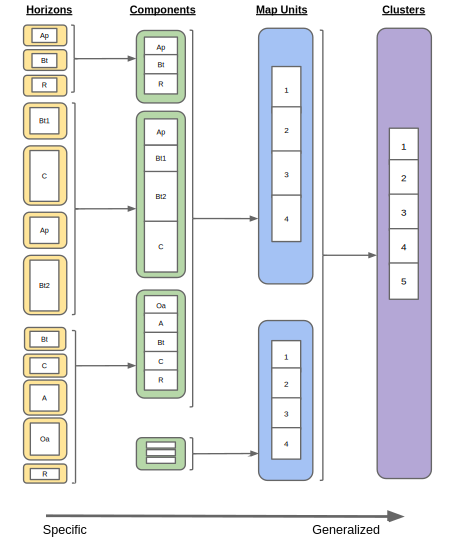
\includegraphics[width=\textwidth]{./img/aggregation_flow_diagram}
	\caption[Flow diagram of the soil aggregation process]{Flow diagram of the soil aggregation process. Horizons are grouped together according to which component they belong. Components are grouped together according to which map unit they  belong. A weighted average is calculated, based upon the component percentage. Mapunits are grouped together according to hydrologic soil group  and are then assigned to a cluster based on a clustering algorithm. Clusters are created by aggregated map units together using a depth-weighted horizon average of soil properties.}
	\label{fig:agg_flow_diagram}
\end{figure}

\begin{figure}[h]
\centering
 \includegraphics[width=0.5\textwidth]{./img/ssurgo_data_structure_schematic.jpeg}
	\caption[Schematic diagram of SSURGO data structure]{Schematic diagram of SSURGO data structure \cite{gatzke_aggregation_2011}}.
	\label{fig:ssurgo_schematic}
\end{figure}

\begin{figure}[h]
  \centering
    \includegraphics[width=0.5\textwidth]{./img/component_schematic.png}
	\caption[Schematic diagram of SSURGO map unit]{Schematic diagram of SSURGO map unit. Antigo and Houghton are each components within the map unit. Within each map unit are varying numbers of components with varying horizon depths (e.g., Ap and O1 are the surface horizons for Antigo and Houghton respectively. Components were aggregated to map units by averaging soil properties (e.g., percent sand) horizontally across horizons.}
	\label{fig:component_schematic}
\end{figure}

\clearpage
\begin{figure}[H]
	\centering
	\includegraphics[width=\textwidth]{./img/cluster_variability.png}
	\caption[Boxplots showing the variability of soil properties]{Boxplots showing the variability of soil properties within the final set of soil clusters. The letter above each plot denotes hydrologic soil group (HSG). Each color represents a cluster of map units. The Z score for each soil property is reported as $Z = X - \mu / \sigma$ where $X$ is the value of the soil property, $\mu$ and $\sigma$ are the population mean and standard deviation of a soil property. Outliers were excluded. The x-axis shows soil properties where tot\_depth is the soil depth, sand/silt/clay are the percent composition of each texture class, bd is bulk density, k is saturated conductivity, awc is available water capacity, cbn is organic carbon concentration, and usle\_k is soil erodibility.}
	\label{fig:soil_boxplots}
\end{figure}